\section{Introduction}

\subsection{Background}

The African penguin (\textit{Spheniscus demersus}) is listed as critically endangered, and its
population decline has been linked to the spatial mismatch between breeding colonies and the
location of prey. At sea, penguins forage in groups and appear to use vocal signals to maintain
contact, coordinate diving and recruit conspecifics to feeding aggregations. Unlike visual or
chemical signals, sound propagates over hundreds of metres in the shallow coastal water where
these birds forage, which makes acoustics the plausible channel for group-level coordination.
A conservation programme that wishes to reduce acoustic disturbance therefore needs three
quantities that connect to one another \cite{ref1,ref2,ref3}: the acoustic structure that carries identity and
intent, the physical distance over which that structure survives, and the behavioural
probability that a bird responds once the signal is audible.

The problem supplies exactly these three pieces of evidence, but not their connection.
Acoustic measurements describe what the calls look like; propagation recordings describe how
the signal degrades with distance; playback experiments describe how often penguins react.
Modelling the connection is not a matter of stacking three models. It requires deciding what
counts as ``hearing'', what counts as ``responding'', and how the two should be combined so
that the result can be used to size a protected buffer.

\subsection{Problem restatement}

We are asked to answer four linked questions.

\begin{enumerate}[leftmargin=1.6em,itemsep=2pt]
  \item Characterise the three call types (flat, modulated, two-voice) using the supplied
        acoustic measurements; identify which features separate them; build a classifier and
        use at least two nonparametric tests; and name the key acoustic indicators that later
        questions should carry forward.
  \item Fuse the three propagation correlations into a fidelity measure that varies with
        distance; fit degradation models for each call type; define a graded threshold scheme;
        estimate the effective communication range under two criteria, with uncertainty ranges;
        and conduct sensitivity analyses over thresholds, weights and model families.
  \item Analyse the playback experiments: compare natural calls with controls, relate response
        to context, call type, distance and group size within one modelling framework,
        describe the distribution of the eight possible response combinations, model response
        latency, and produce a numerical table for representative conditions.
  \item Combine fidelity and recruitment probability into a single communication-effectiveness
        index; state its functional form and the ecological interpretation of its weights; use
        it to estimate an effective radius or an expected number of responders; and translate
        the result into conservation recommendations together with the limitations of the data.
\end{enumerate}

\subsection{Approach and contributions}

Our approach follows the causal chain rather than the questionnaire. The contributions we claim
are the following.

\begin{itemize}[leftmargin=1.6em,itemsep=2pt]
  \item \textbf{We treat the playback experiment as a paired design throughout.} The 139
        experiments each contain one natural call and one control under the same date and
        context. Analyses that ignore this structure underestimate the call effect by a factor
        of nearly three (OR 12.4 instead of 37.0) and can make the distance effect disappear
        entirely. Every inferential statement in Section~\ref{sec:q3} is therefore built on
        within-pair contrasts or on clustered estimating equations.
  \item \textbf{We separate physical audibility from behavioural recruitment.} The fidelity
        index $F(d)$ answers ``is the signal still recognisable''; the recruitment probability
        $P_{\mathrm{recruit}}(d)$ answers ``will a bird come''. Their product, not their weighted
        sum, is the quantity a manager needs, because a signal that cannot be heard cannot
        recruit and a signal that is heard need not recruit. This is the index of Section~\ref{sec:q4}.
  \item \textbf{We model non-response as censoring rather than as a zero.} The problem states
        explicitly that no response does not mean no perception. We therefore split the analysis
        into a response probability and a latency model, carry non-responders as right-censored
        observations in the Kaplan--Meier summary, and report both a conditional median (among
        responders) and a restricted mean survival time that keeps non-responders in the
        denominator.
  \item \textbf{We report ranges instead of point values wherever the data support more than
        one defensible model.} Three of the seven analytic choices we examine --- the weight on
        the envelope correlation, the recognition threshold and the family of the decay curve ---
        each move the estimated radius by tens of metres, and in one case reverse the ranking of
        call types. Reporting a single ``true'' radius would misrepresent what is known.
\end{itemize}

Section~\ref{sec:data} describes the data and the assumptions that the rest of the paper depends
on. Sections~\ref{sec:q1}--\ref{sec:q4} answer the four problems. Section~\ref{sec:discussion}
collects the uncertainty analysis and the limitations, and Section~\ref{sec:conclusion} concludes.

\begin{figure}[htbp]
  \centering
  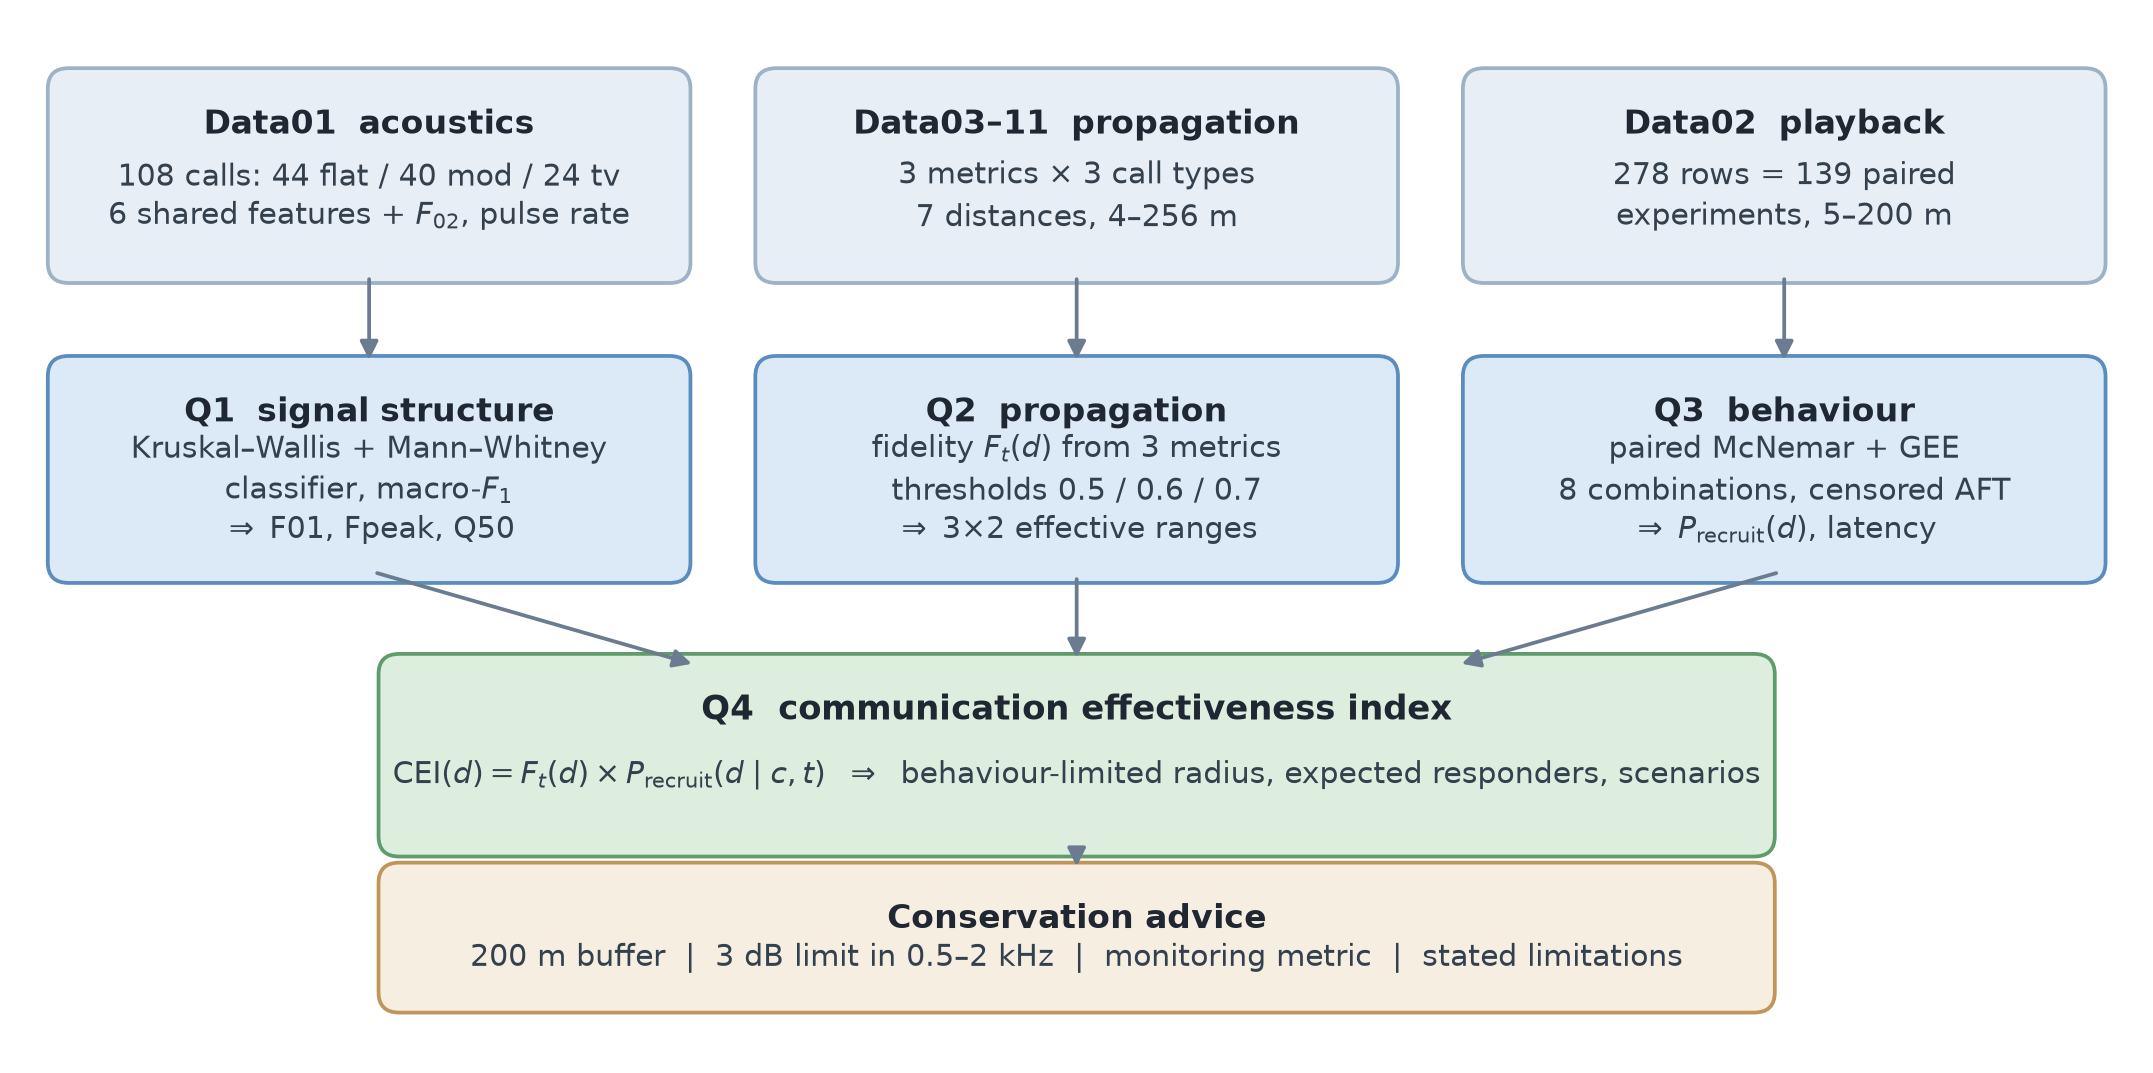
\includegraphics[width=0.80\textwidth]{figs/fig0_route.png}
  \caption{Technical route. Three data sources feed three parallel analyses, which are combined
  into one index and translated into conservation advice.}\label{fig:route}
\end{figure}

The four sections are not four essays; they form one chain, and every link is explicit. Problem~1
returns three spectral indicators (F01, Fpeak, Q50) and the statement that the call types differ
along the frequency axis. Problem~2 returns the fidelity surface $F_t(d)$ built from all three
propagation metrics. Problem~3 returns the recruitment probability
$P_{\mathrm{recruit}}(d\mid c,t)$ and the latency distribution. Problem~4 multiplies the first two
into the index and reads the radii off it. If any link is missing, the next section cannot be
computed: this is why we do not report a single ``combined'' model that would blur the provenance
of each number.
